% -*- TeX:UK -*-
\section{Rotation of factors or components}

\begin{figure}
   \caption{Eigenvectors plotted into the coordinate system of the components obtained. All eigenvectors of \acs{PCA} have unit length and point from the centre to the circumference of a unit circle (sphere or spheroid in higher dimensional cases). Rotation of the coordinate system (\emph{blue arrow}) achieves a structure that is simpler to interpret. The angles between the original and the new coordinate axis are called \(\theta_{xy}, \theta_{xx}, \theta_{yx}, \theta_{yy} \), respectively. They are measured in mathematically positive direction (counterclockwise).}
   \label{fig:RotGeo}
   \centering
      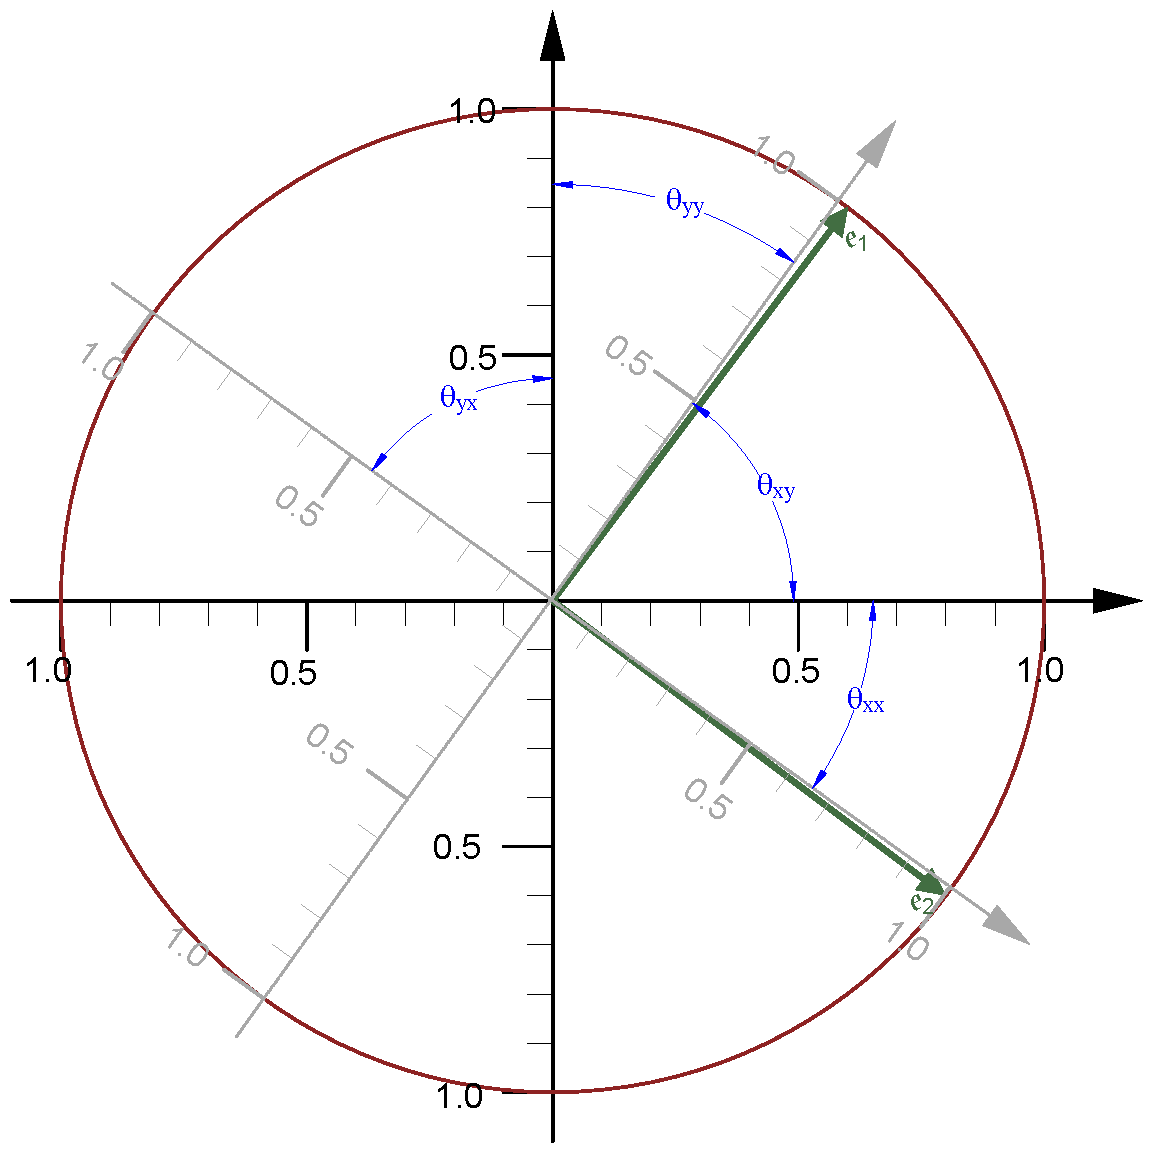
\includegraphics[width=0.75\textwidth]{Graphics/Rotation}
\end{figure}

To make the result of a factor analysis (or \acs{PCA} if it is used as proxy for \acs{FA}) more interpretable the found factors are rotated to achieve a simple structure \parencite{Thur-47}. A simple structure should fulfill the following criteria (for more than four factors extracted):
\begin{itemize}
  \item{each row (variable) contains at least one near zero}
  \item{each column (factor) should have several near zeros}
  \item{for any pair of factors, there are
     \begin{itemize}
       \item{some variables with near zero loadings on one factor and large loadings on the other}
       \item{a sizable number of variables that have near zero loadings on both}
       \item{a small number of variables that have large loadings on both}
     \end{itemize} }
\end{itemize}
Geometrically, the loadings in each row of the loading matrix constitute the coordinates of a point in loading space. If there are clusters of points, we try to put our axes near these clusters, so that each group of variables becomes associated with a factor. If all points are close to an axis, then they would load highly on the corresponding factor, and only little on all others. The complexity of a variable is the number of factors that this variable has moderate or high loadings on. The simple structure then has a complexity of 1.

In other words, the variance of factor loadings per factor is maximised. Note that since rotation is performed only on the factors retained, the result of rotation will change if more or fewer factors are retained. There are two classes of rotation, each with several methods \parencite{Kie-98,Abd-03,Cla-88}:
\begin{description}
  \item[orthogonal]{only right angles between axes are allowed, factors are uncorrelated. The \emph{orthomax function} maximised is \(Q_\mathrm{max}  = \sum_{j,k = 1}^{p, q}{\AbsVec{l}_{jk}^4} - \gamma/p \sum_{k=1}^q{(\sum_{j=1}^p{\AbsVec{l}_{jk}^2})^2} \).
     \begin{description}
        \item[Varimax]{was introduced by \Name{Kaiser} \parencite{Kai-58,Kai-59} and expressed in matrix terms by others \parencite{She-66,Nev-86}. The axes are rotated until all loadings become either large or small, thereby number of variables with high loadings on several factors is minimised. The orthomax function is used with \(\gamma = 1 \). }
        \item[Quartimax]{The number of factors required to explain a variable is minimised, this makes interpretation of the variables easier. The orthomax function is used with \(\gamma = 0 \).}
        \item[Equamax]{is a mixture of Varimax and Quartimax.}
    \end{description} }
  \item[oblique]{angle between axes may be different from \ang{90}, there is correlation between rotated factors. However, this correlation is small, as highly correlated factors would be better interpreted as one factor. Oblique rotations produce two matrices as solution, called pattern and structure matrix, respectively. The most important oblique methods are:
    \begin{description}
        \item[Promax]{is fast and therefore the most frequently used oblique rotation, especially with large data sets. A target matrix is calculated from a varimax rotation whose loadings are raised to a power \(\num{2} < \kappa < \num{4} \), maintaining the sign. This reduces the loadings, but increases the ratio of loadings. Often, an average between the varimax and promax solutions is calculated (procrustean rotation).}
        \item[Oblimin]{produces results that look very much like varimax, except that they are oblique. The degree of obliqueness allowed is controlled by a parameter \textdelta, negative values decrease factor correlation, positive increase it. \(\delta = -4 \) produces uncorrelated factors, default in SPSS is \num{0}, maximum should be \num{0.8} or so. The method minimises the cross-product between loadings, the \emph{oblimin criterium} minimised is \(Q_\mathrm{min} = \sum_{r \neq s}{\left(\sum_{j=1}^p{\AbsVec{l}_{jr}^2\AbsVec{l}_{js}^2} - \gamma/p \sum_{j=1}^p{\AbsVec{l}_{jr}^2} \sum_{j=1}^p{\AbsVec{l}_{js}^2}\right)} \). The special cases of \(\gamma = 0 \) and \(\gamma = 1 \) are called \textbf{quartimin} and \textbf{covarimin}, respectively.}
    \end{description} }
\end{description}
An orthogonal rotation matrix \(\Theta \) is defined, where the rows represent the original and the columns the new  axes \parencite{Abd-03}. Each element of the matrix is the cosine of the angle between the old and new axis, measured in mathematically positive direction (counterclockwise, see fig. \ref{fig:RotGeo})). For the 2D-case:
\begin{gather}
   \Theta = \begin{pmatrix}
                \cos(\theta_{xx}) & \cos(\theta_{xy}) \\
                \cos(\theta_{yx}) & \cos(\theta_{yy}) \\
            \end{pmatrix}
          = \begin{pmatrix}
                \cos(\theta_{xx}) & -\sin(\theta_{xx}) \\
                \sin(\theta_{xx}) &  \cos(\theta_{xx}) \\
            \end{pmatrix}
\end{gather}
This matrix is orthonormal (\( \Theta^T\Theta = \arr{I} \)). The purpose of rotation is to maximise \(Q_\mathrm{max} \) (or minimise \(Q_\mathrm{min} \))

Some authors claim that it is better to perform an oblique rotation first, and a orthogonal only if the resulting angles between factors are not very different from \ang{90} \parencite{Cos-05}. This way, one doesn't enforce a structure which the data don't have. On the other hand, if two factors are correlated (angle significantly different from \ang{90}), then what causes the correlation? In addition, oblique rotation induces additional variability that will make replication of the results in future studies less likely (less factor invariance). The arbitrary setting of \textkappa\ and \textdelta\ by the researcher adds to this problem. The better fit of oblique rotations may be a result of over-fitting. When \acs{PCA} rather than \acs{FA} is used to extract factors, the resulting factors (actually: components) are by definition uncorrelated and oblique rotation will produce similar results to orthogonal.

If there is a strong factor structure in the data, the results from various rotation methods should look similar, if they don't you have a problem anyway. Therefore, the simplest method (varimax) may be used as default.

\begin{figure}
 \caption{Redistribution of explained variance between factors due to rotation. The total explained variance doesn't change, but the relative importance of the components does. }
 \label{fig:trace}
 \centering
 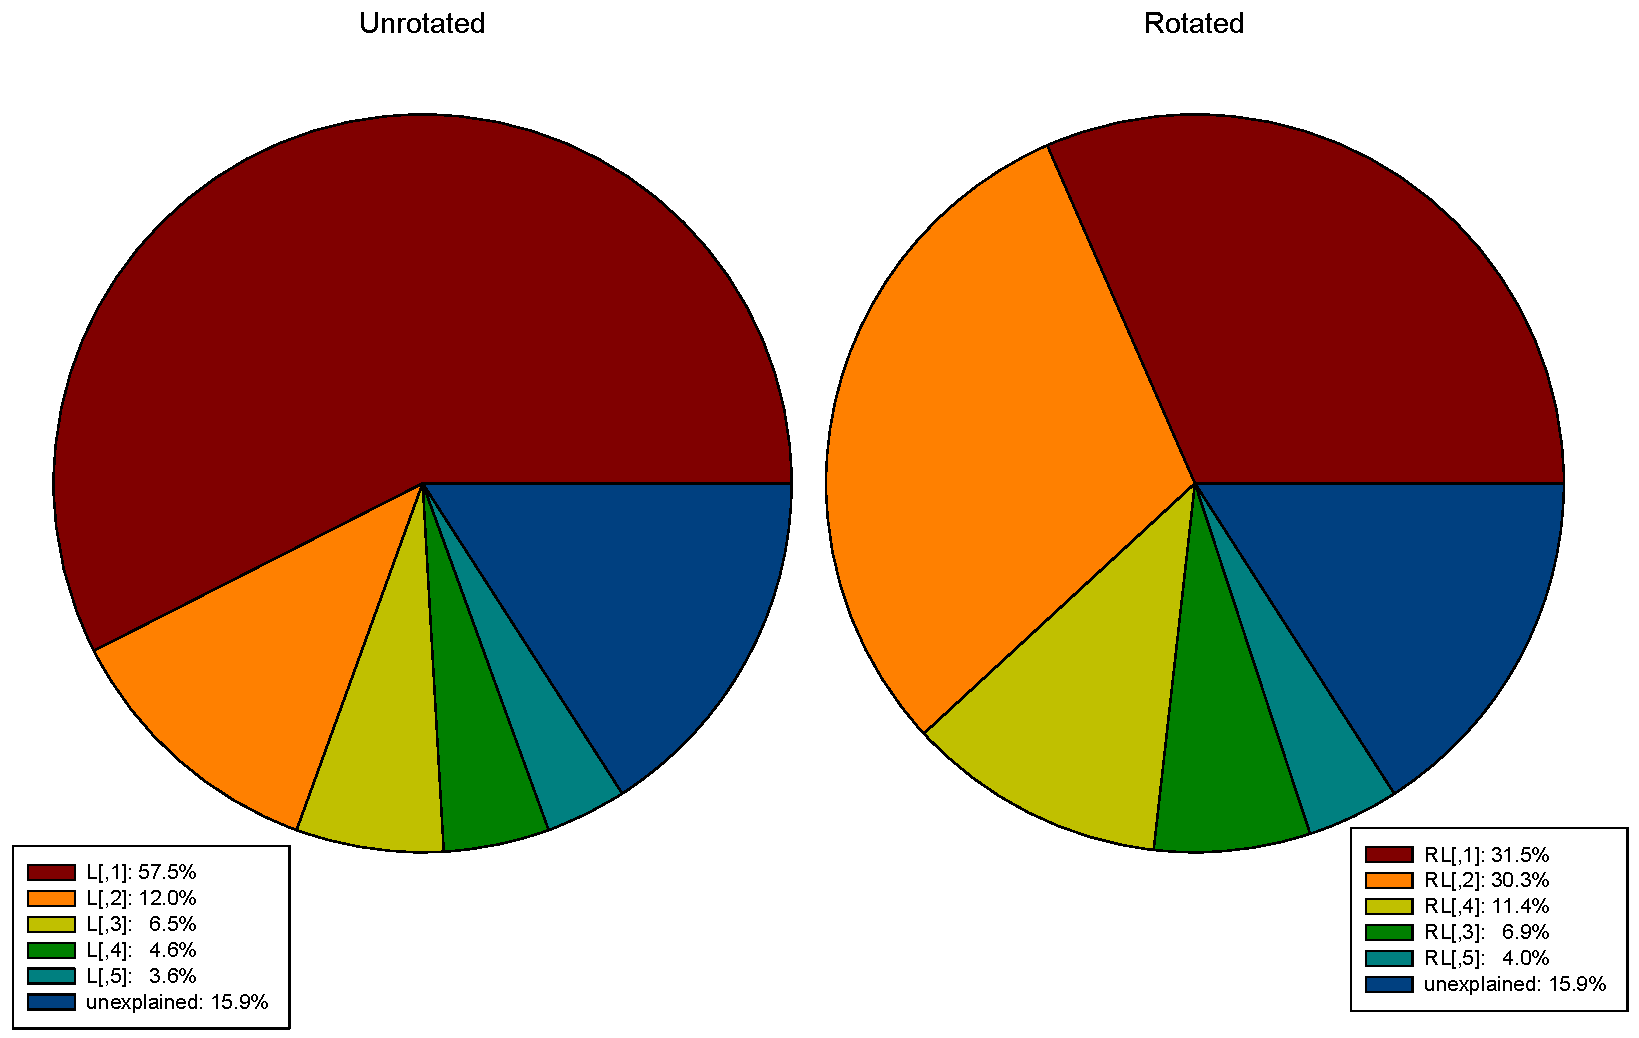
\includegraphics[width=\textwidth]{Graphics/Effect-rotation}
\end{figure}

After rotation, the new loading matrix \arr{L}' reproduce the covariance matrix just like \arr{L}:
\begin{equation}
  \arr{S} = \arr{L}'\arr{L}'^T + \Psi = \arr{L}\theta\theta^T\arr{L}^T  + \Psi = \arr{L}\arr{L}^T  + \Psi
\end{equation}
with \(\Psi_p \) the specific variance. However, the relative importance of factors changes, and is no longer given by the original eigenvalues (see fig. \ref{fig:trace}). A new variance-accounted-for statistics, the \textbf{trace}, is used. After orthogonal rotation, the trace are the column sums of squared factor loadings, and the communalities the row sums (just as in the unrotated case). For oblique rotations, the pattern coefficients are multiplied with the corresponding structure coefficient, the results are summed column-wise for the trace and row-wise for the communalities.

\subsection{Mathematical procedure for orthogonal rotation}

\subsubsection{Gradient projection algorithm (GPA)}\label{text:GPA}

If \arr{L} is the loading matrix, and \( Q_\mathrm{min}(\arr{L}) \) a rotation criterium, then this criterium is to be minimised over all possible rotations, defined in the rotation matrix \( \Theta \). The rotation then becomes \parencite{Jen-01} \( \arr{L}' = \arr{L} \Theta \) and the function to be minimised over all \( \Theta \) is \( f(\Theta) = Q_\mathrm{max}(\arr{L}\Theta) \). For algorithms like varimax, which originally required maximising a quality function, we simply take the negative. The basic algorithm then becomes:
\begin{enumerate}
  \item{Choose an \( \alpha \geq 0 \) and a rotation matrix \( \Theta \) (can be the identity matrix or a random orthogonal matrix) }
  \item{Compute \( \arr{G} = df/d\Theta \), with \( df/d\Theta \) the matrix of partial derivatives }
  \item{Move \( \alpha \) units down the gradient by computing a singular value decomposition \( \arr{U}\Delta\arr{V}^T \) of \( \arr{G} + \alpha\Theta \) }
  \item{Replace \( \Theta \) by \( \arr{UV}^T \)}
  \item{either go to 2) or stop }
\end{enumerate}
This algorithm will converge stationary if \( \alpha \) is sufficiently large. The differential \( \arr{G} = df/d\Theta = \arr{L}^T \frac{dQ}{d\arr{L}'} \) for the quartimax function \(Q(\arr{L}') = 1/4 \sum{\sum{\AbsVec{l}_{jk}^4}} \) becomes \( \frac{dQ}{d\arr{L}'} = \arr{L}'^3 \), which is the element-wise cube of \arr{L}'. For quartimax and varimax rotation, \( \alpha = 0 \) is sufficient to ensure convergence in a few steps. A fixed point of \( \Theta \), that is a \( \Theta \) that doesn't change when the algorithm is applied to it, is also a stationary point of \( f(\Theta) \). It can be shown that with sufficiently large \( \alpha \) the algorithm converges monotonically toward such a fixed point, independently of the starting value of \( \Theta \). As a stationary point is approached, the measure \skalar{v} approaches zero: \(v = ||\mathrm{skm} \Theta^T \arr{G}|| + ||(\arr{I} - \Theta \Theta^T) \arr{G}|| \), where the skew-symmetric part of a square matrix is skm(\arr{M}) = \( 1/2 \arr{M}-(\arr{M})^T \). In practice, one can stop the iteration when \( v \leq \num{e-6} \).

\( \alpha \) needs to be large enough to guarantee monotonicity, but too large an \(\alpha \) will make the algorithm run slower. Operationally, one can run the algorithm with a chosen \( \alpha \) (say, 0) and see if \skalar{v} monotonically declines. If not, \( \alpha \) needs to be increased by some \( \Delta\alpha \) until it does. \parencite{Jen-04,Ber-05} provides more general optimisation criteria, component loss functions that use the second, rather than the fourth, power functions, for example an entropy function \( O(\arr{L}') = -\sum{\sum{\AbsVec{l}^2_{j,k} \log{\AbsVec{l}^2_{j,k}}}} \) that results in simpler \arr{L}' than either quartimax or varimax, small changes in the loading matrix at start produce less big changes in final outcome. Code examples may be found at \parencite{Ber-05a}. An interesting case of rotation are the tandem criteria \parencite{Com-67}: A loading matrix is first rotated by tandem 1 to determine the number of relevant factors, the reduced loading matrix is then rotated by the tandem 2 algorithm.

\begin{sidewaystable}
  \caption{Quality criteria and their differentials, all given for minimisation \parencite{Ber-05}. \( \langle\arr{X,Y}\rangle = \trace(\arr{X}^T \arr{Y}) \) represents the \Name{Frobenius}-scalar product of matrices \( \arr{X}_{n\times p}, \arr{Y}_{n\times p} \), \( \langle\arr{X}\rangle = \langle\arr{X^T,X}\rangle = \sqrt{\sum_{i=1}^m{\sum_{j=1}^n{a_{i,j}^2}}} \) the \Name{Frobenius}-norm of the matrix \( \arr{X} \), \( \arr{X}\odot\arr{Y} \) the element-wise (\Name{Hadamard-Schur}) product and \( \arr{X}^2 = \arr{X}\odot\arr{X} \) the element-wise square of a matrix. \arr{I} is the identity matrix, \arr{N} a (compatible) square matrix with \num{0} in the diagonal, \num{1} everywhere else, and \( \arr{M}_{p\times p} \) a matrix with \( \AbsVec{m}_{ij} = 1/p \). \( \AbsVec{U}_p, \AbsVec{V}_q \) are column vectors of \num{1}.  }
  \label{tab:rot}
  \centering
    \small{\begin{tabular}{lll}
      \toprule
      Criterium                & \( Q_\mathrm{min}(\arr{L}') \)                                                                  & \( \arr{G} = df/d\Theta \)                                                             \\
      \midrule
      quartimax                & \( -1/4 \sum_i{\sum_j{\AbsVec{l}_{ij}}} = -\langle\arr{L}'^2, \arr{L}'^2\rangle/4 \)            & \( -\arr{L}'^3 \)                                                                      \\
      oblimin                  & \( \langle\arr{L}'^2,(\arr{I}-\gamma\arr{M})\arr{L}'^2\arr{N}\rangle / 4 \)                     & \( \arr{L}' \odot [(\arr{I} - \gamma \arr{M})\arr{L}'^2 \arr{N}] \)                    \\
      \Name{Crawford-Ferguson} & \( (1 - \kappa)\langle\arr{L}'^2, \arr{L}'^2 \arr{N} \rangle/4 + \kappa \langle\arr{L}'^2, \arr{N}\arr{L}'^2\rangle/4 \)  & \( (1 - \kappa)\arr{L}' \odot \arr{L}'^2\arr{N} + \kappa\arr{L}' \odot\arr{N}\arr{L}'^2 \) \\
      quartimax                & \grqq, \( \kappa = 0 \)                                                                         & \grqq, \( \kappa = 0 \)                                                                \\
      varimax                  & \grqq, \( \kappa = 1/p \)                                                                       & \grqq, \( \kappa = 1/p \)                                                              \\
      equamax                  & \grqq, \( \kappa = q/2p \)                                                                      & \grqq, \( \kappa = q/2p \)                                                             \\
      parsimax                 & \grqq, \( \kappa = \frac{q-1}{p+q-2} \)                                                         & \grqq, \( \kappa = \frac{q-1}{p+q-2} \)                                                \\
      factor parsimony         & \grqq, \( \kappa = 1 \)                                                                         & \grqq, \( \kappa = 1 \)                                                                \\
      \Name{Jennrich} minimum entropy & \( -\langle\arr{L}'^2, \log\arr{L}'^2\rangle/2 \)                                        & \( -\arr{L}' \odot \log(\arr{L}'^2) - \arr{L}' \)                                      \\
      Oblimax                  & \( -\log\langle\arr{L}'^2\rangle^2 + 2 \log\langle\arr{L}'\rangle^2 \)                          & \( -\frac{4\arr{L}'^3}{\langle\arr{L}'^2\rangle^2} + \frac{4 \arr{L}'}{\langle\arr{L}'\rangle^2} \) \\
      tandem criteria I        & \( -\langle\arr{L}'^2, (\arr{L'}\arr{L}^T)^2\arr{L}'^2\rangle \)                                & \( -4\arr{L}' \odot [(\arr{L}'\arr{L}'^T)^2\arr{L}'^2] \)                              \\
      tandem criteria II       & \( \langle\arr{L}'^2, [\arr{U}\arr{U}^T - (\arr{L}'\arr{L}'^T)^2]\arr{L}'^2\rangle \)           & \( 4\arr{L}' \odot {[\arr{U}\arr{U}^T - ((\arr{L}'\arr{L}'^T)^2)]\arr{L}'^2} - 4{[\arr{L}'\arr{L}'^T] [\arr{L}'^2(\arr{L}'^2)^T]} \arr{L}' \) \\
      \bottomrule
    \end{tabular}}
\end{sidewaystable}

\subsubsection{Penalised varimax}

Interpretation of rotated factors may be complicated by the different communalities of each factor. It is possible to constrain rotation so that communalities are the same for all factors \parencite{Tre}. The varimax rotation does a fairly good job in this respect, which may be one of the reasons for its popularity. It maximises \( Q_\mathrm{max}  = \sum_{j,k = 1}^{p, q}{\AbsVec{l}_{jk}^4} - 1/p \sum_{k=1}^q{\left(\sum_{j=1}^p{\AbsVec{l}_{jk}^2}\right)^2} \). The rotation can be defined in matrix terms
\begin{align}
  \nonumber
  \arr{M}(\Theta) &= \arr{N}^T \arr{O} \arr{N} \\
  \nonumber
  \arr{N} &= \arr{L}' \odot \arr{L}'\\
  \arr{O} &= \arr{I} - \frac{\arr{I}\arr{I}^T}{p}
\end{align}
where \(\odot \) represents the \Name{Hadamard-Schur} (elementwise) product of two matrices. \( \arr{M}/(p-1) \) is the covariance matrix of the squared \arr{L}'. Hence we have to maximise \( \sigma(\Theta) = \mathrm{trace}(\arr{M}(\Theta)) \).
In an orthogonal rotation, the sum of squared loadings is not changed, \( \mathrm{trace}(\arr{L}^T \arr{L}) = \mathrm{trace}(\arr{L}'^T) \arr{L}' =\) const. The requirement that all factors should have equal sums of squares means that \( \arr{L}'^T_{\cdot 1} \arr{L}'_{\cdot 1} = \ldots = \arr{L}'^T_{\cdot q} \arr{L}'_{\cdot q} \). In order to achieve this, the varimax function must be modified with an additional constraint \( PV(\Theta) = \mathrm{trace}(\arr{N})^T \arr{O} \arr{N} - \mu \arr{I}^T \arr{N} \arr{N}^T \arr{I} \) with \skalar{\mu} a  positive number that controls the importance of the penalty term, adjusting the result from pure varimax for \skalar{\mu} = 0  to equal sum of squares for large \skalar{\mu}. The gradient of this function is \( 4 \arr{L}^T {\arr{L}' \odot [(\arr{O} - \mu \arr{I} \arr{I}^T) \arr{N}]} \).

\subsection{Pascal code for rotation}

Rotation of loading matrices is performed by gradient projection according to \parencite{Ber-05}, using  R and SAS example code deposited on \parencite{Ber-05a}. For the time being, only orthogonal rotation is implemented. The rotation methods available are listed in an enumeration type. These can be used by the calling program to specify the desired method:

\begin{lstlisting}[caption=Interface of unit Rotation]
  UNIT Rotation;

  { Rotation of loading matrices by gradient projection according to
    C.A. Bernaards & R.I. Jennrich: Gradient Projection Algorithms and Software
    for Arbitrary Rotation Criteria in Factor Analysis,
    Educ. Psychol. Meas. 65:5 (2005) 676-696, doi:10.1177/0013164404272507.
    Some code in R and SAS is deposited on http://www.stat.ucla.edu/research/gpa/ }

  INTERFACE

  USES MathFunc, Vector, Matrix, SingularValue;

  CONST
    Convergence = -5; // log OF convergence criterium considered success

  TYPE
    RotType = (Varimax, Quartimax, Equamax, Parsimax, Parsimony, Quartimin,
      Biquartimin, Covarimin, Entropy, Tandem1, Tandem2);

  PROCEDURE GradProjAlgOrth(VAR Loading, Rotation: MatrixTyp; RotAlg: RotType);
  { Gradient Projection Algorithm for orthogonal rotation. Rotation algorithm used
    is selected by RotAlg.  }

  PROCEDURE CalculateSAL(CONST Loading: MatrixTyp; VAR SAL: VectorTyp);
  { Sorted absolute loadings (SAL) of a loading matrix. }


  IMPLEMENTATION
\end{lstlisting}

\subsubsection{Rotation methods}

The calculation of the gradient matrix and of the quality measure in each rotation are performed in procedures that depend on the rotation method used.

\paragraph{Varimax}

The varimax method \parencite{Kai-58} is one of the oldest, most used and generally successful rotation methods. As alternative to below procedure the \Name{Crawford-Ferguson}-routine with \(\kappa = 1/p \) may also be used. Varimax is used for orthogonal rotation.

\begin{lstlisting}[caption=Varimax]
  PROCEDURE FVarimax(CONST ActLoading: MatrixTyp; VAR Gradient: MatrixTyp;
    VAR Quality: double);

  VAR
    cm, L2, QL, Zwischen: MatrixTyp;
    n: WORD;

  BEGIN
    HadamardSchurProduct(ActLoading, ActLoading, L2);            // L^2
    n := MatrixRows(L2);
    CreateMatrix(cm, n, n, 1.0 / n);
    MatrixInnerProduct(cm, L2, Zwischen);
    DestroyMatrix(cm);
    NegativeMatrix(Zwischen);
    MatrixAdd(L2, Zwischen, QL);
    DestroyMatrix(L2);
    DestroyMatrix(Zwischen);
    Quality := -FrobeniusNorm(QL) / 4;
    CopyMatrix(ActLoading, Zwischen);
    NegativeMatrix(Zwischen);
    HadamardSchurProduct(Zwischen, QL, Gradient);
    DestroyMatrix(Zwischen);
    DestroyMatrix(QL);
  END;
\end{lstlisting}

\paragraph{Quartimax}

Quartimax is also used for orthogonal rotation. It is less often used than varimax, as it may produce a general factor that loads on most variables. As alternative to below procedure the \Name{Crawford-Ferguson}-routine with \(\kappa = 0 \) may also be used.

\begin{lstlisting}[caption=Quartimax]
  PROCEDURE FQuartimax (CONST ActLoading : MatrixTyp;
                        VAR Gradient : MatrixTyp;
                        VAR Quality : float);

  VAR L2 : MatrixTyp;

  BEGIN
    HadamardSchurProduct(ActLoading, ActLoading, L2);  // L^2
    Quality := -0.25 * sqr(FrobeniusNorm(L2));         // -1/4 <L^2>^2
    HadamardSchurProduct(L2, ActLoading, Gradient);    // L^3
    NegativeMatrix(Gradient);                          // -L^3
    DestroyMatrix(L2);
  END;
\end{lstlisting}


\paragraph{The oblimin family}

Oblimin rotations are used for oblique rotations. Obliqueness is controlled by the parameter \(\gamma \):
\begin{description}
  \item[0.0]{quartimin (most oblique)}
  \item[0.5]{bi-quartimin}
  \item[1.0]{covarimin}
\end{description}

\begin{lstlisting}[caption=Oblimin]
  PROCEDURE FOblimin(CONST ActLoading: MatrixTyp; gamma: double;
    VAR Gradient: MatrixTyp; VAR Quality: double);
  { gamma determines type:
    0.0 quartimin (most oblique)
    0.5 Bi-quartimin
    1.0 covarimin }

  VAR
    Rows, Columns, i, j: WORD;
    Ident, N, M, Zwischen, Zwischen2, L2: MatrixTyp;

  BEGIN
    Rows := MatrixRows(ActLoading);
    Columns := MatrixColumns(ActLoading);
    CreateIdentityMatrix(Ident, Columns);
    NegativeMatrix(Ident);
    CreateMatrix(Zwischen, Columns, Columns, 1.0);
    MatrixAdd(Zwischen, Ident, N);
    DestroyMatrix(Zwischen);
    DestroyMatrix(Ident);
    CreateIdentityMatrix(Ident, Rows);
    FOR i := 1 TO Rows DO
      FOR j := 1 TO Rows DO
        SetMatrixElement(Ident, i, j, GetMatrixElement(Ident, i, j) - gamma);
    CreateMatrix(M, Rows, Rows, 1 / Rows);
    HadamardSchurProduct(ActLoading, ActLoading, L2);            // L^2
    MatrixInnerProduct(L2, N, Zwischen);
    HadamardSchurProduct(Ident, M, Zwischen2);
    DestroyMatrix(Ident);
    DestroyMatrix(M);
    DestroyMatrix(N);
    MatrixInnerProduct(Zwischen2, Zwischen, N);
    // [(I(p)-gamma \cdot M) * L2 * N]
    DestroyMatrix(Zwischen);
    DestroyMatrix(Zwischen2);
    Quality := FrobeniusSkalarProduct(L2, N) / 4;
    // <L2, [(I(p)-gamma \cdot M) * L2 * N]>
    HadamardSchurProduct(ActLoading, N, Gradient);
    // L \cdot [(I(p)-gamma \cdot M) * L2 * N]
    DestroyMatrix(N);
    DestroyMatrix(L2);
  END;
\end{lstlisting}

\paragraph{Entropy}

This method was introduced as alternative to varimax in \parencite{Ber-05}; it gives good results for orthogonal, but poor for oblique rotations.

\begin{lstlisting}[caption=Entropy]
  PROCEDURE FEntropy(CONST ActLoading: MatrixTyp; VAR Gradient: MatrixTyp;
    VAR Quality: double);

  VAR
    L2, lnL2, Zwischen: MatrixTyp;
    i, j: WORD;

  BEGIN
    HadamardSchurProduct(ActLoading, ActLoading, L2);            // L^2
    CopyMatrix(L2, lnL2);
    FOR i := 1 TO MatrixRows(lnL2) DO
      FOR j := 1 TO MatrixColumns(lnL2) DO
        SetMatrixElement(lnL2, i, j, Ln(GetMatrixElement(lnL2, i, j)));
    Quality := -FrobeniusSkalarProduct(L2, lnL2) / 2;          // -<L2, log(L2)>/2
    DestroyMatrix(L2);
    HadamardSchurProduct(ActLoading, lnL2, Zwischen);
    DestroyMatrix(lnL2);
    MatrixAdd(Zwischen, ActLoading, Gradient);            // L \cdot Ln(L2) - L
    NegativeMatrix(Gradient);
    DestroyMatrix(Zwischen);
  END;
\end{lstlisting}

\paragraph{Tandem criteria}

Introduced in \parencite{Com-67}. Criterion I is based upon the principle that variables which appear on the same factor should be correlated and is used to determine the number of relevant factors. Criterion II is based upon the principle that variables which are uncorrelated should not appear on the same factor, and is used to explore factor structure.

\begin{lstlisting}[caption=Tandem criteria]
  PROCEDURE FTandem1(CONST ActLoading: MatrixTyp; VAR Gradient: MatrixTyp;
    VAR Quality: double);

  VAR
    TL, TL2, LL, LL2, L2, gq1, gq2, Zwischen, Zwischen1: MatrixTyp;

  BEGIN
    MatrixTranspose(ActLoading, TL);
    MatrixInnerProduct(ActLoading, TL, LL);
    DestroyMatrix(TL);
    HadamardSchurProduct(LL, LL, LL2);
    HadamardSchurProduct(ActLoading, ActLoading, L2);
    MatrixTranspose(L2, TL2);
    MatrixInnerProduct(LL2, L2, Zwischen);
    DestroyMatrix(LL2);
    MatrixInnerProduct(TL2, Zwischen, Zwischen1);
    Quality := -MatrixTrace(Zwischen1);
    DestroyMatrix(Zwischen1);
    HadamardSchurProduct(ActLoading, Zwischen, gq1);
    SkalarMultiplikation(gq1, 4);
    DestroyMatrix(Zwischen);
    MatrixInnerProduct(L2, TL2, Zwischen);
    DestroyMatrix(TL2);
    DestroyMatrix(L2);
    HadamardSchurProduct(LL, Zwischen, Zwischen1);
    DestroyMatrix(LL);
    DestroyMatrix(Zwischen);
    MatrixInnerProduct(Zwischen1, ActLoading, gq2);
    SkalarMultiplikation(gq2, 4);
    DestroyMatrix(Zwischen1);
    NegativeMatrix(gq1);
    NegativeMatrix(gq2);
    MatrixAdd(gq1, gq2, Gradient);
    DestroyMatrix(gq1);
    DestroyMatrix(gq2);
  END;


  PROCEDURE FTandem2(CONST ActLoading: MatrixTyp; VAR Gradient: MatrixTyp;
    VAR Quality: double);

  VAR
    TL, TL2, LL, LL2, L2, U, TU, UU, gq1, gq2,
    Zwischen, Zwischen1, Copy                       : MatrixTyp;
    p: WORD;

  BEGIN
    p := MatrixRows(ActLoading);
    MatrixTranspose(ActLoading, TL);
    MatrixInnerProduct(ActLoading, TL, LL);
    DestroyMatrix(TL);
    HadamardSchurProduct(LL, LL, LL2);
    NegativeMatrix(LL2);
    DestroyMatrix(LL);
    CopyMatrix(ActLoading, Copy);
    HadamardSchurProduct(Copy, Copy, L2);
    CreateMatrix(U, p, 1, 1.0);
    CreateMatrix(TU, 1, p, 1.0);
    MatrixInnerProduct(U, TU, UU);
    DestroyMatrix(U);
    DestroyMatrix(TU);
    MatrixAdd(UU, LL2, Zwischen);
    DestroyMatrix(UU);
    MatrixInnerProduct(Zwischen, L2, Zwischen1);
    Quality := FrobeniusSkalarProduct(L2, Zwischen1);
    SkalarMultiplikation(Copy, 4);
    HadamardSchurProduct(Copy, Zwischen1, gq1);   {******}
    DestroyMatrix(Copy);
    DestroyMatrix(Zwischen);
    DestroyMatrix(Zwischen1);
    MatrixTranspose(L2, TL2);
    MatrixInnerProduct(L2, TL2, Zwischen);
    DestroyMatrix(L2);
    DestroyMatrix(TL2);
    HadamardSchurProduct(LL2, Zwischen, Zwischen1);
    DestroyMatrix(Zwischen);
    DestroyMatrix(LL2);
    MatrixInnerProduct(Zwischen1, Copy, gq2);
    DestroyMatrix(Zwischen1);
    SkalarMultiplikation(gq2, -4);
    MatrixAdd(gq1, gq2, Gradient);
    DestroyMatrix(gq1);
    DestroyMatrix(gq2);
  END;
\end{lstlisting}

\paragraph{\Name{Crawford-Ferguson}}

This is a general method for orthogonal rotation \parencite{Craw-70}, that depending on the parameter \(\kappa \) performs like
\begin{description}
  \item[0]{Quartimax}
  \item[\( 1/p \)]{Varimax}
  \item[\( q/(2*p) \)]{Equamax}
  \item[\( (q-1)/(p+q-2) \)]{Parsimax}
  \item[1]{Factor parsimony}
\end{description}

\begin{lstlisting}[caption=\Name{Crawford-Ferguson}]
  PROCEDURE FCrawfordFerguson(CONST ActLoading: MatrixTyp; kappa: double;
    VAR Gradient: MatrixTyp; VAR Quality: double);

  VAR
    Rows, Columns: WORD;
    Ident, N, M, Zwischen, L2, g1, g2: MatrixTyp;
    f1, f2: double;

  BEGIN
    Rows := MatrixRows(ActLoading);
    Columns := MatrixColumns(ActLoading);
    CreateIdentityMatrix(Ident, Columns);
    NegativeMatrix(Ident);
    CreateMatrix(Zwischen, Columns, Columns, 1.0);
    MatrixAdd(Zwischen, Ident, N);
    DestroyMatrix(Ident);
    DestroyMatrix(Zwischen);
    CreateIdentityMatrix(Ident, Rows);
    NegativeMatrix(Ident);
    CreateMatrix(Zwischen, Rows, Rows, 1.0);
    MatrixAdd(Zwischen, Ident, M);
    DestroyMatrix(Ident);
    DestroyMatrix(Zwischen);
    HadamardSchurProduct(ActLoading, ActLoading, L2);            // L^2
    MatrixInnerProduct(L2, N, Zwischen);
    f1 := (1 - kappa) * FrobeniusSkalarProduct(L2, Zwischen) / 4;
    // (1-kappa) <L2, (L2*N)> /4
    HadamardSchurProduct(ActLoading, Zwischen, g1);             // L \cdot (L2 * N)
    DestroyMatrix(Zwischen);
    DestroyMatrix(N);
    MatrixInnerProduct(M, L2, Zwischen);
    f2 := kappa * FrobeniusSkalarProduct(L2, Zwischen) / 4;      // kappa * <L2, (M*L2)> /4
    HadamardSchurProduct(ActLoading, Zwischen, g2);             // L \cdot (M * L2)
    DestroyMatrix(Zwischen);
    DestroyMatrix(M);
    Quality := f1 + f2;
    SkalarMultiplikation(g1, 1 - kappa);
    SkalarMultiplikation(g2, kappa);
    MatrixAdd(g1, g2, Gradient);
    DestroyMatrix(L2);
    DestroyMatrix(g1);
    DestroyMatrix(g2);
  END;
\end{lstlisting}

\paragraph{\Name{Bendler}'s method} \parencite{Ben-77}:

\begin{lstlisting}[caption=\Name{Bendler}]
  PROCEDURE FBentler(CONST ActLoading: MatrixTyp; VAR Gradient: MatrixTyp;
    VAR Quality: double);     // funktioniert nicht

  VAR
    L2, TL2, M, D, Zwischen, Zwischen1: MatrixTyp;
    Det1, Det2: double;

  BEGIN
    HadamardSchurProduct(ActLoading, ActLoading, L2);
    MatrixTranspose(L2, TL2);
    MatrixInnerProduct(TL2, L2, M);
    DestroyMatrix(TL2);
    CopyMatrix(M, D);
    Det1 := Determinante(D);
    Diag(D);
    Det2 := Determinante(D);
    Quality := -Ln(Det1 / Det2);
    InverseMatrix(M);
    InverseMatrix(D);
    MatrixInnerProduct(M, D, Zwischen);
    DestroyMatrix(M);
    DestroyMatrix(D);
    MatrixInnerProduct(L2, Zwischen, Zwischen1);
    DestroyMatrix(L2);
    DestroyMatrix(Zwischen);
    CopyMatrix(Zwischen1, Zwischen);
    SkalarMultiplikation(Zwischen, -4);
    HadamardSchurProduct(Zwischen, Zwischen1, Gradient);
    DestroyMatrix(Zwischen);
    DestroyMatrix(Zwischen1);
  END;
\end{lstlisting}


\subsubsection{Gradient projection algorithm for orthogonal rotation}


\begin{lstlisting}[caption=Implementation of the gradient projection algorithm for orthogonal rotation]
PROCEDURE GradProjAlgOrth(VAR Loading, Rotation: MatrixTyp; RotAlg: RotType);

VAR
  alpha, s, s1, Q, Qold: double;
  Columns, Rows, j, Iter: WORD;
  NewLoading, LoadingTrans, RotationTrans, GradQ, Grad, GradP,
  Manifold, ManifoldTrans, Zwischen, Skm2, X, V, VT: MatrixTyp;
  Delta: VectorTyp;

BEGIN
  alpha := 1.0;
  Columns := MatrixColumns(Loading);
  Rows := MatrixRows(Loading);
  Writeln;
  Writeln('Rotation:');
  Writeln('Iter Q      s           Log10(s)  alpha ');
  MatrixInnerProduct(Loading, Rotation, NewLoading);
  CreateMatrix(GradQ, Columns, Columns, 0.0);
  CASE RotAlg OF
    Varimax: FCrawfordFerguson(NewLoading, 1 / Rows, GradQ, Q);
    Quartimax: FCrawfordFerguson(NewLoading, 0.0, GradQ, Q);
    Equamax: FCrawfordFerguson(NewLoading, Columns / (2 * Rows), GradQ, Q);
    Parsimax: FCrawfordFerguson(NewLoading, Pred(Columns) /
        (Rows + Columns - 2), GradQ, Q);
    Parsimony: FCrawfordFerguson(NewLoading, 1.0, GradQ, Q);
    Quartimin: FOblimin(NewLoading, 0.0, GradQ, Q);
    Biquartimin: FOblimin(NewLoading, 0.5, GradQ, Q);
    Covarimin: FOblimin(NewLoading, 1.0, GradQ, Q);
    Entropy: FEntropy(NewLoading, GradQ, Q);
    Tandem1: FTandem1(NewLoading, GradQ, Q);
    Tandem2: FTandem2(NewLoading, GradQ, Q);
    //    Bentler    : FBentler(NewLoading, GradQ, Q);
  END;
  Qold := Q;
  MatrixTranspose(Loading, LoadingTrans);
  MatrixInnerProduct(LoadingTrans, GradQ, Grad);    // calculate gradient
  Iter := 0;
  REPEAT
    MatrixTranspose(Rotation, RotationTrans);
    MatrixInnerProduct(RotationTrans, Grad, Manifold);        // M = T' * G
    MatrixTranspose(Manifold, ManifoldTrans);
    MatrixAdd(Manifold, ManifoldTrans, Skm2);
    SkalarMultiplikation(Skm2, 0.5);                      // S = (M+M')/2
    MatrixInnerProduct(Rotation, Skm2, Zwischen);
    DestroyMatrix(Skm2);
    NegativeMatrix(Zwischen);
    MatrixAdd(Grad, Zwischen, GradP);                     // Gp = G - T*S
    DestroyMatrix(Zwischen);
    s := FrobeniusNorm(GradP);
    s1 := log(s, 10);
    Writeln(Iter: 3, '  ', Q: 2: 3, ' ', s: 2: 8, ' ', s1: 2: 3, '     ', alpha: 2: 2);
    IF (s1 > Convergence)
      THEN
        BEGIN
          alpha := 2 * alpha;
          j := 0;
          REPEAT                                             // ensure that Q IS decreased
            DestroyMatrix(NewLoading);
            SkalarMultiplikation(GradP, -alpha);
            MatrixAdd(Rotation, GradP, X);          // X = T - a1*Gp
            SVDCmp(X, Delta, V);                             // X now contains U
            MatrixTranspose(V, Vt);
            DestroyMatrix(V);
            MatrixInnerProduct(X, Vt, Zwischen);               // Tt = U T'
            MatrixInnerProduct(Loading, Zwischen, NewLoading); // L = A * Tt
            CASE RotAlg OF
              Quartimax: FCrawfordFerguson(NewLoading, 0.0, GradQ, Q);
              Varimax: FCrawfordFerguson(NewLoading, 1 / Rows, GradQ, Q);
              Equamax: FCrawfordFerguson(NewLoading, Columns / (2 * Rows), GradQ, Q);
              Parsimax: FCrawfordFerguson(NewLoading, pred(Columns) /
                  (Rows + Columns - 2), GradQ, Q);
              Parsimony: FCrawfordFerguson(NewLoading, 1.0, GradQ, Q);
              Quartimin: FOblimin(NewLoading, 0.0, GradQ, Q);
              Biquartimin: FOblimin(NewLoading, 0.5, GradQ, Q);
              Covarimin: FOblimin(NewLoading, 1.0, GradQ, Q);
              Entropy: FEntropy(NewLoading, GradQ, Q);
              Tandem1: FTandem1(NewLoading, GradQ, Q);
              Tandem2: FTandem2(NewLoading, GradQ, Q);
              //              Bentler    : FBentler(NewLoading, GradQ, Q);
            END;
            IF (Q > (Qold - 0.5 * s * s * alpha)) 
              THEN alpha := alpha / 2;
            Inc(j);
            DestroyMatrix(X);
            DestroyMatrix(Vt);
            DestroyVector(Delta);
          UNTIL ((j = 10) OR (Q < (Qold - 0.5 * s * s * alpha)));
          CopyMatrix(Zwischen, Rotation);
          DestroyMatrix(Zwischen);
        END;
    Qold := Q;
    MatrixInnerProduct(LoadingTrans, GradQ, Grad);
    Inc(Iter);
    DestroyMatrix(RotationTrans);
    DestroyMatrix(Manifold);
    DestroyMatrix(ManifoldTrans);
  UNTIL ((s1 < Convergence) OR (Iter > MaxIter));
  DestroyMatrix(NewLoading);
  MatrixInnerProduct(Loading, Rotation, NewLoading);
  DestroyMatrix(Loading);
  CopyMatrix(NewLoading, Loading);
  DestroyMatrix(NewLoading);
  DestroyMatrix(LoadingTrans);
  DestroyMatrix(GradQ);
  DestroyMatrix(GradP);
  DestroyMatrix(Grad);
END;
\end{lstlisting}

\subsubsection{Sorted absolute loadings}

The sorted absolute loadings (SAL) of a loading matrix can be used for a SAL-plot \parencite{Ber-05}, which is a simple method to see how well the rotation worked. SAL plotted versus number should result in a sigmoidal function.

\begin{lstlisting}[caption=Calculation of SAL]
  PROCEDURE CalculateSAL(CONST Loading: MatrixTyp; VAR SAL: VectorTyp);

  VAR
    i, j, Rows, Columns, Length: word;

  BEGIN
    Rows := MatrixRows(Loading);
    Columns := MatrixColumns(Loading);
    Length := Rows * Columns;
    CreateVector(SAL, Length, 0.0);
    FOR i := 1 TO Rows DO
      FOR j := 1 TO Columns DO
        SetVectorElement(SAL, i * j, abs(GetMatrixElement(Loading, i, j)));
    Shellsort(SAL);
  END;

  END.
\end{lstlisting}

\subsection{Examples}

\subsubsection{\Name{Thurstone}'s box problem}

The initial loading matrix \arr{L} of \Name{Thurstone}'s box problem is:

\begin{tabular}{rrrr}
  \toprule
   \# & 1     & 2      &  3     \\
  \midrule
   1 & 0.659 & -0.736 &  0.138 \\
   2 & 0.725 &  0.180 & -0.656 \\
   3 & 0.665 &  0.537 &  0.500 \\
   4 & 0.869 & -0.209 & -0.443 \\
   5 & 0.834 &  0.182 &  0.508 \\
   6 & 0.836 &  0.519 &  0.152 \\
   7 & 0.856 & -0.452 & -0.269 \\
   8 & 0.848 & -0.426 &  0.320 \\
   9 & 0.861 &  0.416 & -0.299 \\
  10 & 0.880 & -0.341 & -0.354 \\
  11 & 0.889 & -0.417 &  0.436 \\
  12 & 0.875 &  0.485 & -0.093 \\
  13 & 0.667 & -0.725 &  0.109 \\
  14 & 0.717 &  0.246 & -0.619 \\
  15 & 0.634 &  0.501 &  0.522 \\
  16 & 0.936 &  0.257 &  0.165 \\
  17 & 0.966 & -0.239 & -0.083 \\
  18 & 0.625 & -0.720 &  0.166 \\
  19 & 0.702 &  0.112 & -0.650 \\
  20 & 0.664 &  0.536 &  0.488 \\
  \bottomrule
\end{tabular}

Using quartimax rotation and the \(\arr{I}_3 \) as initial rotation matrix the iteration should converge as follows

\begin{tabular}{rrrr}
  \toprule
   iter   & f         & log10    &  alpha  \\
  \midrule
   0      &  -10.7152 &  -0.1406 &  1.0000 \\
   1.0000 &  -13.2425 &   0.3893 &  2.0000 \\
   2.0000 &  -14.1458 &   0.0407 &  0.2500 \\
   3.0000 &  -14.1964 &  -0.4122 &  0.0625 \\
   4.0000 &  -14.2029 &  -0.7978 &  0.0625 \\
   5.0000 &  -14.2041 &  -1.0890 &  0.0625 \\
   6.0000 &  -14.2046 &  -1.6858 &  0.1250 \\
   7.0000 &  -14.2046 &  -2.2221 &  0.1250 \\
   8.0000 &  -14.2046 &  -2.5689 &  0.0625 \\
   9.0000 &  -14.2046 &  -3.1207 &  0.1250 \\
  10.0000 &  -14.2046 &  -3.4477 &  0.0625 \\
  11.0000 &  -14.2046 &  -4.0147 &  0.1250 \\
  12.0000 &  -14.2046 &  -4.3231 &  0.0625 \\
  13.0000 &  -14.2046 &  -4.9043 &  0.1250 \\
  14.0000 &  -14.2046 &  -5.1958 &  0.0625 \\
  \bottomrule
\end{tabular}

The rotation matrix \(\theta \) becomes

\begin{tabular}{rrrr}
  \toprule
   1     & 2       & 3       \\
  \midrule
  0.5723 & -0.6075 & -0.5508 \\
  0.6025 &  0.7672 & -0.2201 \\
  0.5563 & -0.2059 &  0.8051 \\
  \bottomrule
\end{tabular}

The final loading matrix \arr{L}' is (\( |\AbsVec{l}| > 0.7 \) in red, \(< 0.3 \) in blue):

\begin{tabular}{rrrr}
  \toprule
   \# & 1      & 2       &  3     \\
  \midrule
   1 & \textcolor{blue}{0.0105}& \textcolor{red}{-0.9934} & \textcolor{blue}{-0.0899} \\
   2 & \textcolor{blue}{0.1585}& \textcolor{blue}{-0.1673}& \textcolor{red}{-0.9671} \\
   3 & \textcolor{red}{0.9823} & \textcolor{blue}{-0.0950}& \textcolor{blue}{-0.0819} \\
   4 & \textcolor{blue}{0.1250}& -0.5971                  & \textcolor{red}{-0.7893} \\
   5 & \textcolor{red}{0.8696} & -0.4716                  & \textcolor{blue}{-0.0904} \\
   6 & \textcolor{red}{0.8757} & \textcolor{blue}{-0.1410}& -0.4523 \\
   7 & \textcolor{blue}{0.0679}& \textcolor{red}{-0.8114} & -0.5886 \\
   8 & 0.4067                  & \textcolor{red}{-0.9079} & \textcolor{blue}{-0.1157} \\
   9 & 0.5771                  & \textcolor{blue}{-0.1424}& \textcolor{red}{-0.8065} \\
  10 & \textcolor{blue}{0.1013}& \textcolor{red}{-0.7233} & -0.6946 \\
  11 & 0.5001                  & \textcolor{red}{-0.9497} & \textcolor{blue}{-0.0468} \\
  12 & \textcolor{red}{0.7413} & \textcolor{blue}{-0.1403}& -0.6636 \\
  13 & \textcolor{blue}{0.0056}& \textcolor{red}{-0.9838} & \textcolor{blue}{-0.1200} \\
  14 & \textcolor{blue}{0.2142}& \textcolor{blue}{-0.1194}& \textcolor{red}{-0.9474} \\
  15 & \textcolor{red}{0.9551} & \textcolor{blue}{-0.1083}& \textcolor{blue}{-0.0392} \\
  16 & \textcolor{red}{0.7823} & -0.4054                  & -0.4393 \\
  17 & 0.3627                  & \textcolor{red}{-0.7531} & -0.5463 \\
  18 & \textcolor{blue}{0.0162}& \textcolor{red}{-0.9662} & \textcolor{blue}{-0.0521} \\
  19 & \textcolor{blue}{0.1077}& \textcolor{blue}{-0.2067}& \textcolor{red}{-0.9346} \\
  20 & \textcolor{red}{0.9744} & \textcolor{blue}{-0.0926}& \textcolor{blue}{-0.0908} \\
  \bottomrule
\end{tabular}

\subsubsection{Football players}

Table \ref{tab:football} lists data collected by \Name{G.R.Bryce} and \Name{R.M.Barker} (Brigham Young University) as part of a preliminary study of a possible link between football helmet design and neck injuries:

\begin{center}
  \label{tab:football}
  \tablefirsthead{\toprule Group & WDIM & CIRCUM & FBEYE & EYEHD & EARHD & JAW \\ \midrule}
  \tablehead{\midrule \multicolumn{7}{l} continued from previous page\\ \midrule}
  \tabletail{\midrule \multicolumn{7}{l} continued on next page\\ \midrule}
  \tablelasttail{\bottomrule}
  \topcaption{WDIM = head width at widest dimension, CIRCUM  =  head circumference, FBEYE = front-to-back measurement at eye level, EYEHD = eye-to-top-of-head measurement, EARHD = ear-to-top-of-head measurement, JAW = jaw width. Group 2: college players Group 3: college non-players.}
    \centering
    \begin{supertabular}{rrrrrrr}
      2     & 15.5 & 60.0   & 21.1  & 10.3  & 13.4  & 12.4  \\
      2     & 15.4 & 59.7   & 20.0  & 12.8  & 14.5  & 11.3  \\
      2     & 15.1 & 59.7   & 20.2  & 11.4  & 14.1  & 12.1  \\
      2     & 14.3 & 56.9   & 18.9  & 11.0  & 13.4  & 11.0  \\
      2     & 14.8 & 58.0   & 20.1  &  9.6  & 11.1  & 11.7  \\
      2     & 15.2 & 57.5   & 18.5  &  9.9  & 12.8  & 11.4  \\
      2     & 15.4 & 58.0   & 20.8  & 10.2  & 12.8  & 11.9  \\
      2     & 16.3 & 58.0   & 20.1  &  8.8  & 13.0  & 12.9  \\
      2     & 15.5 & 57.0   & 19.6  & 10.5  & 13.9  & 11.8  \\
      2     & 15.0 & 56.5   & 19.6  & 10.4  & 14.5  & 12.0  \\
      2     & 15.5 & 57.2   & 20.0  & 11.2  & 13.4  & 12.4  \\
      2     & 15.5 & 56.5   & 19.8  &  9.2  & 12.8  & 12.2  \\
      2     & 15.7 & 57.5   & 19.8  & 11.8  & 12.6  & 12.5  \\
      2     & 14.4 & 57.0   & 20.4  & 10.2  & 12.7  & 12.3  \\
      2     & 14.9 & 54.8   & 18.5  & 11.2  & 13.8  & 11.3  \\
      2     & 16.5 & 59.8   & 20.2  &  9.4  & 14.3  & 12.2  \\
      2     & 15.5 & 56.1   & 18.8  &  9.8  & 13.8  & 12.6  \\
      2     & 15.3 & 55.0   & 19.0  & 10.1  & 14.2  & 11.6  \\
      2     & 14.5 & 55.6   & 19.3  & 12.0  & 12.6  & 11.6  \\
      2     & 15.5 & 56.5   & 20.0  &  9.9  & 13.4  & 11.5  \\
      2     & 15.2 & 55.0   & 19.3  &  9.9  & 14.4  & 11.9  \\
      2     & 15.3 & 56.5   & 19.3  &  9.1  & 12.8  & 11.7  \\
      2     & 15.3 & 56.8   & 20.2  &  8.6  & 14.2  & 11.5  \\
      2     & 15.8 & 55.5   & 19.2  &  8.2  & 13.0  & 12.6  \\
      2     & 14.8 & 57.0   & 20.2  &  9.8  & 13.8  & 10.5  \\
      2     & 15.2 & 56.9   & 19.1  &  9.6  & 13.0  & 11.2  \\
      2     & 15.9 & 58.8   & 21.0  &  8.6  & 13.5  & 11.8  \\
      2     & 15.5 & 57.3   & 20.1  &  9.6  & 14.1  & 12.3  \\
      2     & 16.5 & 58.0   & 19.5  &  9.0  & 13.9  & 13.3  \\
      2     & 17.3 & 62.6   & 21.5  & 10.3  & 13.8  & 12.8  \\
      3     & 14.9 & 56.5   & 20.4  &  7.4  & 13.0  & 12.0  \\
      3     & 15.4 & 57.5   & 19.5  & 10.5  & 13.8  & 11.5  \\
      3     & 15.3 & 55.4   & 19.2  &  9.7  & 13.3  & 11.5  \\
      3     & 14.6 & 56.0   & 19.8  &  8.5  & 12.0  & 11.5  \\
      3     & 16.2 & 56.5   & 19.5  & 11.5  & 14.5  & 11.8  \\
      3     & 14.6 & 58.0   & 19.9  & 13.0  & 13.4  & 11.5  \\
      3     & 15.9 & 56.7   & 18.7  & 10.8  & 12.8  & 12.6  \\
      3     & 14.7 & 55.8   & 18.7  & 11.1  & 13.9  & 11.2  \\
      3     & 15.5 & 58.5   & 19.4  & 11.5  & 13.4  & 11.9  \\
      3     & 16.1 & 60.0   & 20.3  & 10.6  & 13.7  & 12.2  \\
      3     & 15.2 & 57.8   & 19.9  & 10.4  & 13.5  & 11.4  \\
      3     & 15.1 & 56.0   & 19.4  & 10.0  & 13.1  & 10.9  \\
      3     & 15.9 & 59.8   & 20.5  & 12.0  & 13.6  & 11.5  \\
      3     & 16.1 & 57.7   & 19.7  & 10.2  & 13.6  & 11.5  \\
      3     & 15.7 & 58.7   & 20.7  & 11.3  & 13.6  & 11.3  \\
      3     & 15.3 & 56.9   & 19.6  & 10.5  & 13.5  & 12.1  \\
      3     & 15.3 & 56.9   & 19.5  &  9.9  & 14.0  & 12.1  \\
      3     & 15.2 & 58.0   & 20.6  & 11.0  & 15.1  & 11.7  \\
      3     & 16.6 & 59.3   & 19.9  & 12.1  & 14.6  & 12.1  \\
      3     & 15.5 & 58.2   & 19.7  & 11.7  & 13.8  & 12.1  \\
      3     & 15.8 & 57.5   & 18.9  & 11.8  & 14.7  & 11.8  \\
      3     & 16.0 & 57.2   & 19.8  & 10.8  & 13.9  & 12.0  \\
      3     & 15.4 & 57.0   & 19.8  & 11.3  & 14.0  & 11.4  \\
      3     & 16.0 & 59.2   & 20.8  & 10.4  & 13.8  & 12.2  \\
      3     & 15.4 & 57.6   & 19.6  & 10.2  & 13.9  & 11.7  \\
      3     & 15.8 & 60.3   & 20.8  & 12.4  & 13.4  & 12.1  \\
      3     & 15.4 & 55.0   & 18.8  & 10.7  & 14.2  & 10.8  \\
      3     & 15.5 & 58.4   & 19.8  & 13.1  & 14.5  & 11.7  \\
      3     & 15.7 & 59.0   & 20.4  & 12.1  & 13.0  & 12.7  \\
      3     & 17.3 & 61.7   & 20.7  & 11.9  & 13.3  & 13.3  \\
      \midrule
 \(\bar{\AbsVec{X}}_{i\cdot} \)   & 15.5 &  57.6 & 19.8 & 10.5 & 13.6 & 11.9 \\
 \(\sigma(\AbsVec{X}_{i\cdot}) \) &  0.6 &   1.6 &  0.7 &  1.2 &  0.7 &  0.6 \\
      \bottomrule
  \end{supertabular}
\end{center}

The var-covariance matrix and correlation matrix are:
\begin{gather} \arr{S} =
   \begin{pmatrix}
   0.3702 & 0.6020 & 0.1488 & 0.0444 &  0.1071 &  0.2093 \\
   0.6020 & 2.6530 & 0.8083 & 0.6645 &  0.1019 &  0.3796 \\
   0.1488 & 0.8083 & 0.4583 & 0.0113 & -0.0132 &  0.1198 \\
   0.0444 & 0.6645 & 0.0113 & 1.4740 &  0.2522 & -0.0544 \\
   0.1071 & 0.1019 & 0.0132 & 0.2522 &  0.4880 & -0.0356 \\
   0.2093 & 0.3796 & 0.1198 & 0.0544 & -0.0356 &  0.3237 \\
   \end{pmatrix} \\
 \arr{R} =
   \begin{pmatrix}
   1.0000 &  0.6075 &  0.3613 &  0.0601 &  0.2520 &  0.6047 \\
   0.6075 &  1.0000 &  0.7331 &  0.3361 &  0.0895 &  0.4097 \\
   0.3613 &  0.7331 &  1.0000 &  0.0137 & -0.0280 &  0.3112 \\
  -0.0601 &  0.3361 &  0.0137 &  1.0000 &  0.2974 & -0.0787 \\
   0.2520 &  0.0895 & -0.0280 &  0.2974 &  1.0000 & -0.0896 \\
   0.6047 &  0.4097 &  0.3112 & -0.0787 & -0.0896 &  1.0000 \\
   \end{pmatrix}
\end{gather}

\Name{Bartlett}'s sphere test shows that both matrices \arr{S} and \arr{R} are significantly different from the identity matrix \arr{I}:

\begin{tabular}{rrrrr}
  \toprule
  Matrix  & Det   & \(\chi^2 \) & \(f \) & \(P_0 \) \\
  \midrule
  \arr{S} & 0.010 & 112.8 & 15 & \(< \SI{0.1}{\%} \) \\
  \arr{R} & 0.094 &  57.8 & 15 & \(< \SI{0.1}{\%} \) \\
  \bottomrule
\end{tabular}
\vspace{5mm}

Eigenvalues from \arr{S} and \arr{R} (see also fig. \ref{fig:Scree-football}):

\begin{tabular}{rrr|rrr}
  \toprule
  EV     & Variance & Cum Var & EV & Variance & Cum Var\\
  \midrule
  3.3450 & 0.5800 & 0.5800 & 2.5680 & 0.4280 & 0.4280 \\
  1.3770 & 0.2388 & 0.8188 & 1.3690 & 0.2281 & 0.6561 \\
  0.4764 & 0.0826 & 0.9014 & 0.9338 & 0.1556 & 0.8117 \\
  0.3252 & 0.0564 & 0.9578 & 0.6780 & 0.1130 & 0.9247 \\
  0.1550 & 0.0269 & 0.9846 & 0.3209 & 0.0535 & 0.9782 \\
  0.0886 & 0.0154 & 1.0000 & 0.1310 & 0.0218 & 1.0000 \\
  \bottomrule
\end{tabular}
\vspace{5mm}

Total variance of \arr{S} \(= \sum_{j=1}^6{\AbsVec{s}_{jj}} = \sum_{j=1}^6{\lambda_j} = 5.77 \). The first two eigenvalues account for \SI{81.8}{\%} of variance. Total variance of \arr{R} \(= \sum_{j=1}^6{\skalar{r}_{jj}} = \sum_{j=1}^6{\lambda_j} = 6.00 \). However, the first two eigenvalues account for only \SI{65.6}{\%} of the variance. Relevant eigenvectors and loadings from \arr{S}:

\begin{tabular}{rrrrrrr}
  \toprule
         & \(\AbsVec{e}_1 \) & \(\AbsVec{e}_2 \) & \(\AbsVec{l}_1 \) & \(\AbsVec{l}_2 \) & Commun & Uniq \\
  \midrule
  WDIM   & 0.0783 & -0.2200 & 0.6199 & -0.2680 & 0.4561 & 0.5439 \\
  CIRCUM & 0.7415 & -0.5191 & 0.9819 & -0.1560 & 0.9884 & 0.0116 \\
  FBEYE  & 0.2153 & -0.2626 & 0.7072 & -0.3979 & 0.6585 & 0.3415 \\
  EYEHD  & 0.5601 &  0.7260 & 0.4852 &  0.8630 & 0.9801 & 0.0199 \\
  EARHD  & 0.2568 &  0.2667 & 0.1690 &  0.3739 & 0.1684 & 0.8316 \\
  JAW    & 0.1344 & -0.1224 & 0.4115 & -0.3825 & 0.3156 & 0.6844 \\
  \midrule
  var acc&        &         & 2.2818 &  1.2854 & 3.5672	& 2.4329 \\
  prop var&       &         & 0.3803 &  0.2142 & 0.5945	& 0.4055 \\
  \bottomrule
\end{tabular}
\vspace{5mm}

\begin{figure}
   \caption{Scree-plot of the football data. }
   \label{fig:Scree-football}
   \centering
      \includegraphics[width=0.75\textwidth]{Graphics/Scree-football}
\end{figure}
\vspace{5mm}

Relevant eigenvectors and loadings from \arr{R}:

\begin{tabular}{rrrrrrr}
  \toprule
         & \(\AbsVec{e}_1 \) & \(\AbsVec{e}_2 \) & \(\AbsVec{l}_1 \) & \(\AbsVec{l}_2 \) & Commun & Uniq \\
  \midrule
  WDIM   & 0.0783 & -0.2200 & 0.7429 &  0.0817 & 0.5586 & 0.4414 \\
  CIRCUM & 0.7415 & -0.5191 & 0.9634 &  0.2677 & 0.9998 & 0.0002 \\
  FBEYE  & 0.2153 & -0.2626 & 0.7538 & -0.0536 & 0.5711 & 0.4289 \\
  EYEHD  & 0.5601 &  0.7260 & 0.3271 &  0.9018 & 0.9202 & 0.0798 \\
  EARHD  & 0.2568 &  0.2667 & 0.1659 &  0.6505 & 0.4507 & 0.5493 \\
  JAW    & 0.1344 & -0.1224 & 0.5661 & -0.2453 & 0.3807 & 0.6193 \\
  \midrule
  var acc&        &         & 2.5032 &  1.3778 & 3.8811	& 2.1189 \\
  prop var&       &         & 0.4172 &  0.2296 & 0.6469	& 0.3532 \\
  \bottomrule
\end{tabular}
\vspace{5mm}

\begin{figure}
   \caption{The scores resulting from the football data }
   \label{fig:Scores-football}
   \centering
      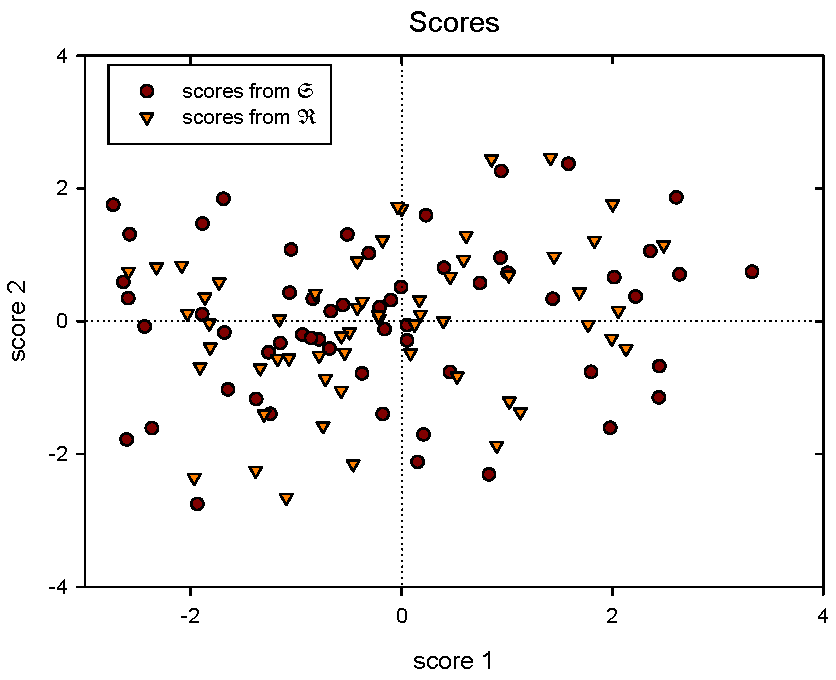
\includegraphics[width=0.75\textwidth]{Graphics/Scores-football}
\end{figure}

\vspace{5mm}

Varimax-rotation of these loadings proceeds in 5 steps for \arr{S} and 12 steps for \arr{R}. \\

{\footnotesize \begin{tabular}{r|rrrr|rrrr}
  \toprule
           & \multicolumn{4}{l} \arr{S} &  \multicolumn{4}{l} \arr{R}  \\
           & \(\AbsVec{l}_1 \) & \(\AbsVec{l}_2 \) & Commun & Uniq & \(\AbsVec{l}_1 \) & \(\AbsVec{l}_2 \) & Commun & Uniq \\
  \midrule
  WDIM     & 0.6753 & -0.0030 & 0.4561 & 0.5439  & 0.7289 &  0.1650 & 0.5586 & 0.4414 \\
  CIRCUM   & 0.9643 &  0.2421 & 0.9884 & 0.0116  & 0.9271 &  0.3746 & 0.9998 & 0.0002 \\
  FBEYE    & 0.8067 & -0.0882 & 0.6585 & 0.3415  & 0.7551 &  0.0318 & 0.5711 & 0.4289 \\
  EYEHD    & 0.1073 &  0.9842 & 0.9801 & 0.0199  & 0.2233 &  0.9329 & 0.9202 & 0.0798 \\
  EARHD    & 0.0086 &  0.4102 & 0.1684 & 0.8316  & 0.0915 &  0.6651 & 0.4507 & 0.5493 \\
  JAW      & 0.5286 & -0.1901 & 0.3156 & 0.6844  & 0.5902 & -0.1799 & 0.3807 & 0.6193 \\
  \midrule
  var acc  & 2.3277 &  1.2395 & 3.5672 & 2.4329  & 2.3676 &  1.5136 & 3.8811 & 2.1189 \\
  prop var & 0.3880 &  0.2066 & 0.5945 & 0.4055  & 0.3946 &  0.2523 & 0.6469 & 0.3532 \\
  \bottomrule
\end{tabular}}

\begin{figure}
   \caption{Unrotated and rotated loadings from the football-data }
   \label{fig:Loadings-football}
   \centering
      \includegraphics[width=0.75\textwidth]{Graphics/Loadings-football}
\end{figure}


\subsection{Interpretation}

How many variables should be included when interpreting a factor? According to \parencite{Gua-88} the following rules are supported by Monte Carlo simulation:
\begin{itemize}
  \item{when at least 4 variables load on a factor with at least 0.60, sample size is of little consequence}
  \item{when at least 10 variables load on a factor with at least 0.40, sample size is of little consequence}
  \item{If these conditions are not met, sample size should be at least 300}
  \item{If sample size is less than 300, random loading patterns may become relevant. The study should be reproduced. }
\end{itemize}

\printbibliography[heading=subbibliography]
\end{refsection}

